%%%%%%%%%%%%%%%%%%%%%%%%%%%%%%%%%%%%%%%%%%%%%%%%%%%%%%%%%%%%%%%%%%%%%%%%%%%%%%%%%%
%                                NO MODIFICAR                                    %
%%%%%%%%%%%%%%%%%%%%%%%%%%%%%%%%%%%%%%%%%%%%%%%%%%%%%%%%%%%%%%%%%%%%%%%%%%%%%%%%%%
\documentclass[11pt,                                                            
%preprint,linenumbers, 
 superscriptaddress,twoside,
 amsmath,amssymb,
 aps, physrev
]{revtex4-2}
\usepackage[utf8]{inputenc}
\usepackage[spanish]{babel}
\usepackage{graphicx}
\usepackage{geometry}
\usepackage{booktabs}
\usepackage{float}
\usepackage{csquotes}
\usepackage{titlesec}
\usepackage{fancyhdr}
\usepackage{lipsum}
\geometry{margin=2cm, 
          top=2.5cm, 
          bottom=2.5cm,
          headheight=15pt,
          includehead,
          }
\titleformat{\section}
  {\normalfont\bfseries} 
  {\thesection.}         
  {1em}                  
  {\raggedright}         
\pagestyle{fancy}
\fancyhf{}
\fancyfoot[C]{\small Capítulo Libro}
\fancyfoot[RE]{\thepage} 
\fancyfoot[LO]{\thepage}
\fancyhead[CO]{\small K.M. GOMEZ M}
\fancyhead[CE]{\small TÍTULO}
\renewcommand{\headrulewidth}{0pt}
\renewcommand{\andname}{y} % comentar si la publicación es en inglés
\fancypagestyle{portada}{
    \fancyhf{}
    \fancyhead[R]{\small Capítulo Libro}
}
%%%%%%%%%%%%%%%%%%%%%%%%%%%%%%%%%%%%%%%%%%%%%%%%%%%%%%%%%%%%%%%%%%%%%%%%%%%%%%%%%%
%%%%%%%%%%%%%%%%%%%%%%%%%%%%%%%%%%%%%%%%%%%%%%%%%%%%%%%%%%%%%%%%%%%%%%%%%%%%%%%%%%



\begin{document}
%%%%%%%%%%%%%%%%%%%%%%%
% Lista de autoras/es %
%%%%%%%%%%%%%%%%%%%%%%%
\title{TÍTULO}
\author{Nombre}
\email{correo@ucr.ac.cr} % Corresponding author
\affiliation{Facultad de Ciencias, Universidad de Costa Rica, San José, Costa Rica}

\author{Nombre}
\affiliation{Centro de Investigación en Ciencias, Universidad de Costa Rica, San José, Costa Rica}

\author{Nombre}
\affiliation{Facultad de Ciencias, Universidad de Costa Rica, San José, Costa Rica}
\affiliation{Centro de Investigación en Ciencias, Universidad de Costa Rica, San José, Costa Rica}


\begin{abstract}
\begin{center}
    {\scriptsize }
\end{center}
{\fontsize{9pt}{11pt}\selectfont


%%%%%%%%%%%%
% Abstract %
%%%%%%%%%%%%
\centering{{\bf Abstract}} 

\textbf{Key words:} 

%%%%%%%%%%%
% Resumen %
%%%%%%%%%%%
\centering{{\bf Resumen}} 
\lipsum[2] \\ % Borre esta línea e incluya aquí el Resumen en español
\textbf{Palabras clave:} 

{\textbf{DOI:} 10.XXXXX/xxxxxxxx} % Se agregará por parte de la Revista
\par}
\end{abstract}
\maketitle
\thispagestyle{portada}

%%%%%%%%%%%%%%%%%%%%%%%%
% Empieza el documento %
%%%%%%%%%%%%%%%%%%%%%%%%
\section{INTRODUCCIÓN}
Revisar cientificos que han publicado y con que razones. 
\subsection{Expertos o teóricos en comunicación pública de la ciencia}

Stephen Hilgartner

La ciencia que aparece en medios no es simplemente una versión simplificada de la ciencia original. Es una versión construida donde se selecciona qué información mostrar y cómo presentarla.

**Idea clave:** la divulgación científica no es neutral; implica decisiones, énfasis y, en muchos casos, intereses.

---
Massimiano Bucchi

La ciencia adopta formas distintas según el público al que se dirige. No se comunica igual entre especialistas que hacia el público general.

**Idea clave:** la ciencia no se “degrada” al comunicarse, sino que se transforma según el contexto y la audiencia.

IDEA estudio: sobre como estudiar a quienes no se interesan en ciencia. 

---

Martin W. Bauer

La relación del público con la ciencia no depende solo del nivel de conocimiento. Factores como la confianza, los valores y el contexto social son fundamentales.

**Idea clave:** el público no es simplemente ignorante; interpreta la ciencia desde sus propios marcos de referencia.

---
Bruce Lewenstein

Existen distintos modelos de comunicación de la ciencia. El más antiguo asumía que el público carece de conocimiento y debe ser instruido, pero enfoques más recientes destacan la importancia del diálogo y la participación.

**Idea clave:** la comunicación de la ciencia no debe ser un proceso unidireccional, sino interactivo.

---
Síntesis general

En conjunto, estos autores coinciden en que la comunicación pública de la ciencia no es un proceso simple de transmisión de información. Implica transformación del conocimiento, interpretación por parte del público y dinámicas sociales donde intervienen factores culturales, políticos y de confianza.

----

Además de Stephen Hilgartner, Massimiano Bucchi, Martin W. Bauer y Bruce Lewenstein, hay varios autores clave que han estructurado el campo de la comunicación pública de la ciencia. Te los organizo por enfoques para que veas mejor el panorama:

---
1. Enfoque crítico y sociológico (ciencia, poder y discurso)

* Brian Wynne
Estudia cómo el conocimiento local y la experiencia del público pueden ser tan válidos como el conocimiento científico.
**Clave:** la ciencia no tiene el monopolio del saber.

* Alan Irwin
Introduce el concepto de **“ciencia ciudadana”**.
**Clave:** los ciudadanos deben participar en decisiones científicas.

* Sheila Jasanoff
Trabaja la relación entre ciencia, política y sociedad.
**Clave:** la ciencia y el orden social se construyen juntos (“coproducción”).

---
2. Public Understanding of Science (PUS) y percepción pública

* John D. Miller
Mide alfabetización científica en distintos países.
**Clave:** cuánto sabe la gente sobre ciencia.

* Nick Pidgeon
Analiza cómo las personas perciben riesgos científicos (ej. cambio climático, energía nuclear).
**Clave:** la percepción del riesgo no es solo racional.

* George Gaskell
Trabaja con encuestas europeas sobre opinión pública.
**Clave:** actitudes hacia la ciencia dependen del contexto cultural.

---

3. Medios, framing y comunicación estratégica

* Matthew Nisbet
Propone el uso de **framing** (encuadres) para comunicar ciencia.
**Clave:** cómo se presenta un tema cambia cómo se entiende.

* Dietram A. Scheufele
Estudia efectos de medios y opinión pública.
**Clave:** la comunicación influye en actitudes, no solo en conocimiento.

---

4. Modelos participativos y engagement

* Rikard Stengler
Analiza la evolución hacia modelos participativos.
**Clave:** involucrar al público en vez de solo informarlo.

* Sarah Davies
Estudia cultura científica y engagement.
**Clave:** la comunicación es también una práctica cultural.

---

5. Divulgación, cultura científica y práctica profesional

* Jay Rosen
Aunque no es exclusivo de ciencia, influye en periodismo participativo.
**Clave:** el público también produce y valida información.

* Naomi Oreskes
Analiza controversias científicas (clima, negacionismo).
**Clave:** la desinformación también es parte de la comunicación científica.

---

Síntesis rápida

El campo se puede leer en tres grandes líneas:

1. **Crítica (STS):** la ciencia es social y política
2. **Percepción pública (PUS):** cómo piensa la gente sobre ciencia
3. **Comunicación estratégica:** cómo presentar la ciencia eficazmente


\url{https://scholar.google.com/citations?view_op=search_authors&hl=en&mauthors=label:public_understanding_of_science}
\subsection{Martin W. Bauer}
\begin{itemize}
	\item Más citado en Google Scholar en tema: Public Understanding of Science.
	\item Es uno de los editores de la revista Public Understanding of Science
	\item Tiene capítulo (cap 14) en libro Routledge Handbook of Public Communication of Science and Technology editado por Massimiano Bucchi y Brian Trench
	\item Nota: Ver libro \cite{Bucchi2021}, Ver capítulo: Public understanding of science: Survey research around the world Martin W. Bauer and Bankole A. Falade
	\item Editor del libro Science Cultures in a Diverse
	World: Knowing, Sharing, Caring
	\item Algunos papers interesantes desde el 2021:
	
	\begin{itemize}
		\item \cite{Massarani2021} 2021 En este artículo muestran los resultados de un estudio a través de encuestas a periodistas científicos durante la pandemia. Hablan del hacer del periodismo científico. Algunas conclusiones del artículo hablan de un aumento en la carga laboral durante este período, de como estos accedían a la información y lidiaban con las noticias falsas, ya que la desinformación en temas de salud afecta la percepción del riesgo y el comportamiento público.
		
		\item \cite{Joubert2023} 2923 Estudian la visibilidad de los científicos durante la pandemia. Comentan las funciones sociales de los científicos más visibles y la ambigüedad que los afecta al querer satisfacer las demandas del público mientras trabajan profesionalmente en la ciencia. Muestran las características de los científicos mas visibles como la edad, el género, la reputación, la imagen pública agradable, el bucle de retroalimentación de la visibilidad, comprensión de los medios de comunicación, estilo accesible, controversia, etc. Discuten estas características para científicos con alta visibilidad durante el COVID-19.
		\item 2023 Libro Science communication : taking a step back to move forward.
		\item \cite{Entradas2023} 2023 Papel de las universidades en la comunicación de la ciencia. Presentan tendencias generales en la comunicación científica de las universidades en  distintos países europeos. Estudian la presencia de personal para la comunicación, financiación, políticas, canales, el público objetivo, la orientación (bien público o interés propio). Concluyen que esto suele ser secundario para las universidades.
		\item 2024 Capitulo de libro. AI with common sense: What concept of common sense?. Tiene otros papers sobre sentido común.
		\item 2024 \cite{Ansell2024} Estudio longitudinal en Reino Unido que busca responder si estrategias nacionalistas de parte de las autoridades públicas, afectan los niveles de vacunación. Descubren que no y que pueden ser contraproducentes.
		\item 2024 \cite{Sammut2024} Examinan (en una población particular) como las cosmovisiones pueden afectar en la recepción de políticas públicas y en la participación de los ciudadanos en estas. Luego es importante para las autoridades políticas conocer las características psicológicas de su público.
		\item 2024 \cite{Oliveira2024} Proponen combinar prácticas de ciencia abierta y comunicación cientifica para promover tanto acceso al material cientifico como su comprensión. Hablan de herramientas puente para abordar la complejidad del léxico y los procesos cientificos. 
		\item 2025 \cite{Hall2025} Estudia como las personas que creen en teorías conspirativas sostienen dichas creencias. Analizan la coexistencia de estas con explicaciones no conspirativas.
		\item 2025 \cite{Bauer2025} Discusión sobre el sentido común y las culturas cientificas. Concluye que la comunicación cientifica no puede limitarse a ser propaganda contra la desinformación y el desmonte de supersticiones populares porque crea rupturas afectando la legitimidad hacia la ciencia por una cultura en particular.
		\item 2026 \cite{BehmBahtat2026} Reflexiones sobre las encuestas para medir la confianza en la ciencia, desde como se operacionaliza el concepto hasta como se redactan las preguntas. Analizan el Eurobarómetro. 
		
	\end{itemize}
	
	\item Algunos de los papers más citados:
	\begin{itemize}
		\item 2007 \cite{Bauer2007} Temas importantes en PUS de los 25 años anteriores a este artículo. Tres paradigmas: Alfabetización científica, comprensión pública de la ciencia, y ciencia y sociedad.
		\item Del 2009 tiene un paper sobre la evolución del campo PUS. También ha estudiado el tema de representaciones sociales. 
	\end{itemize} 
	
	
\end{itemize}



\subsection{Dominique Brossard}
Algunos artículos:
\begin{itemize}
	\item 2025 \cite{Villanueva2025} Los organoides cerebrales humanos son modelos tridimensionales (3D) de "minicerebros" cultivados en laboratorio a partir de células madre pluripotentes inducidas (iPSC). 
	Entonces en este artículo presentan discusión sobre los debates que estos generan en el público. Exploran los valores y las vías cognitivas que dan forma a la opinión en este tema, el cual genera dilemas morales. 
	\begin{quote}
		"La teoría del ciclo de atención a los problemas, propuesta por Downs (1972) , sostiene que la cobertura de temas científicos atraviesa cinco etapas. La primera es la etapa previa al problema, en la que el público general aún no es consciente del problema, aunque algunos expertos o grupos de interés ya han estado atentos al surgimiento de la tecnología. Durante la segunda etapa, o la etapa de "descubrimiento alarmante y entusiasmo eufórico", ocurre un evento que lleva el tema a la conciencia colectiva. En este momento, las personas se preocupan por el problema, pero al mismo tiempo son optimistas sobre la capacidad de la sociedad para resolverlo. La tercera etapa se produce cuando las personas se dan cuenta de que existe un alto costo asociado con la solución del problema, generalmente un costo que no están dispuestas a pagar. Con el tiempo, este pesimismo se transforma en la cuarta etapa, en la que el público general pierde gradualmente el interés debido al aburrimiento, el desánimo o la sensación de agobio. La etapa final se produce cuando el problema es desplazado por otros temas importantes que acaban de entrar en la segunda etapa."
	\end{quote}
	Factores en la formación de actitudes hacia las tecnologías emergentes: Ideología politica, religión, respeto a la ciencia, disposiciones cognitivas y percepción de riesgo, interacciones entre predisposiciones de valores.
	
	\item 2025 \cite{Bao2025} Análisis de segmentación sistemática que compara los riesgos y beneficios percibidos de la IA entre científicos y el público general en EEUU. Algunos factores estudiados: Predisposiciones de valores, creencias previas sobre la ciencia,  las noticias y representaciones de la ciencia en los medios de comunicación. Hallazgos revelan que los científicos de IA generalmente perciben mayores beneficios de la IA que el público general, mientras que ambos grupos muestran niveles similares de riesgos percibidos.
	\item 2025 \cite{Beets2025} Investigan a través de encuestas a profesores universitarios la tendencia a la participación pública de los cientificos. Observan 5 dimensiones de participación: investigación pública o divulgación científica, actividades educativas, interacción directa con el público, colaboración centrada en las partes interesadas y colaboración con la industria. 
\end{itemize}


\subsection{Bruce Lewenstein}


\section{MÉTODOS}

\section{RESULTADOS Y DISCUSIÓN}

Total fragmentos: 62651

Total fragmentos ciencia: 7267

Total framgmentos adminitración de la ciencia: 3195


\begin{figure}[H]
	\centering
	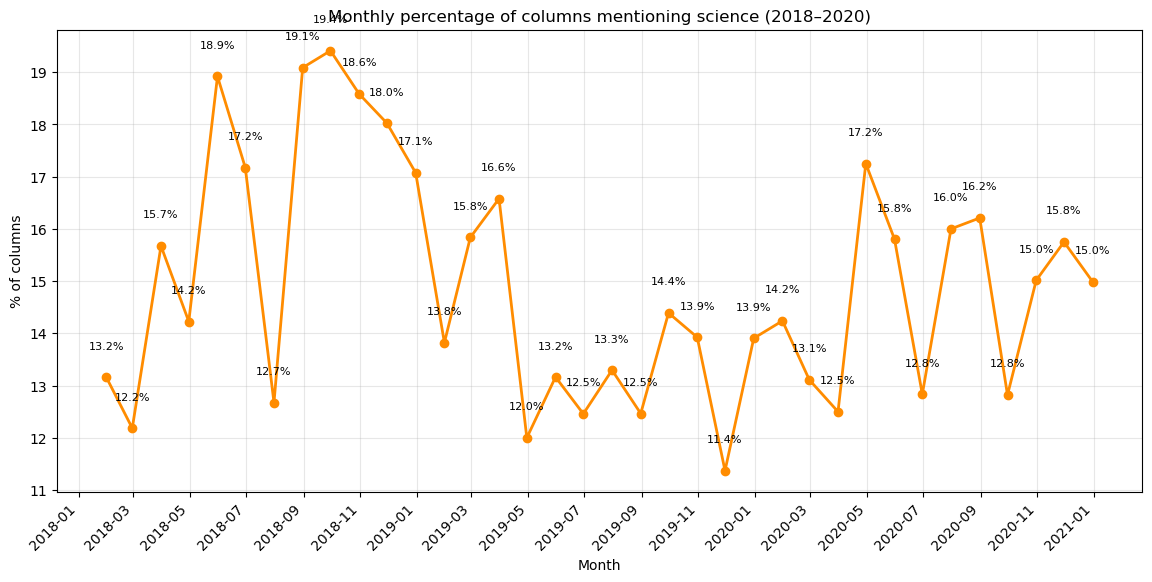
\includegraphics[width=0.8\textwidth]{monthly_percentage.png}
	\caption{Descripción de la imagen}
	\label{fig:monthly_admin_science}
\end{figure}

\begin{figure}[H]
	\centering
	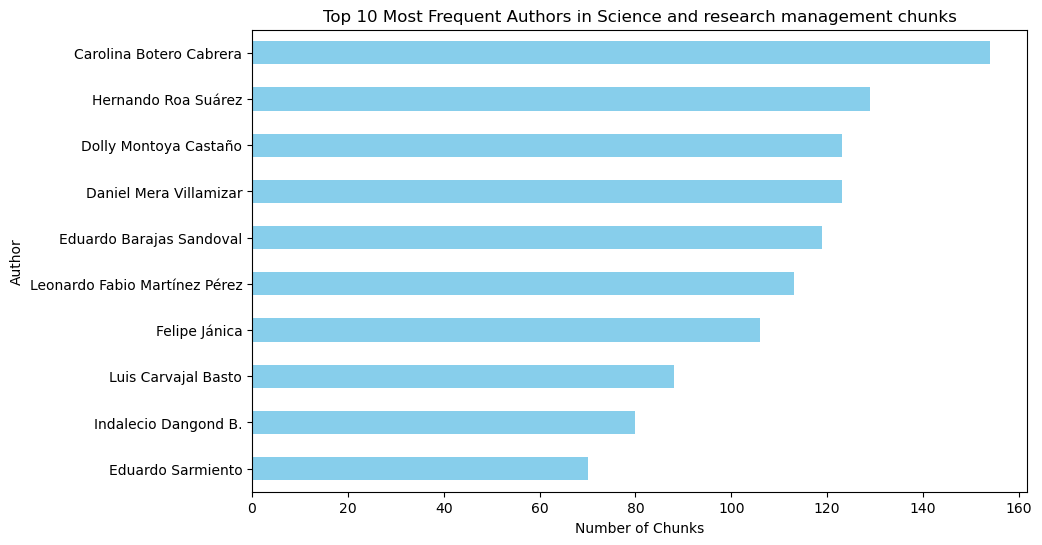
\includegraphics[width=0.8\textwidth]{authors.png}
	\caption{Descripción de la imagen}
	\label{fig:authors}
\end{figure}

\begin{figure}[H]
	\centering
	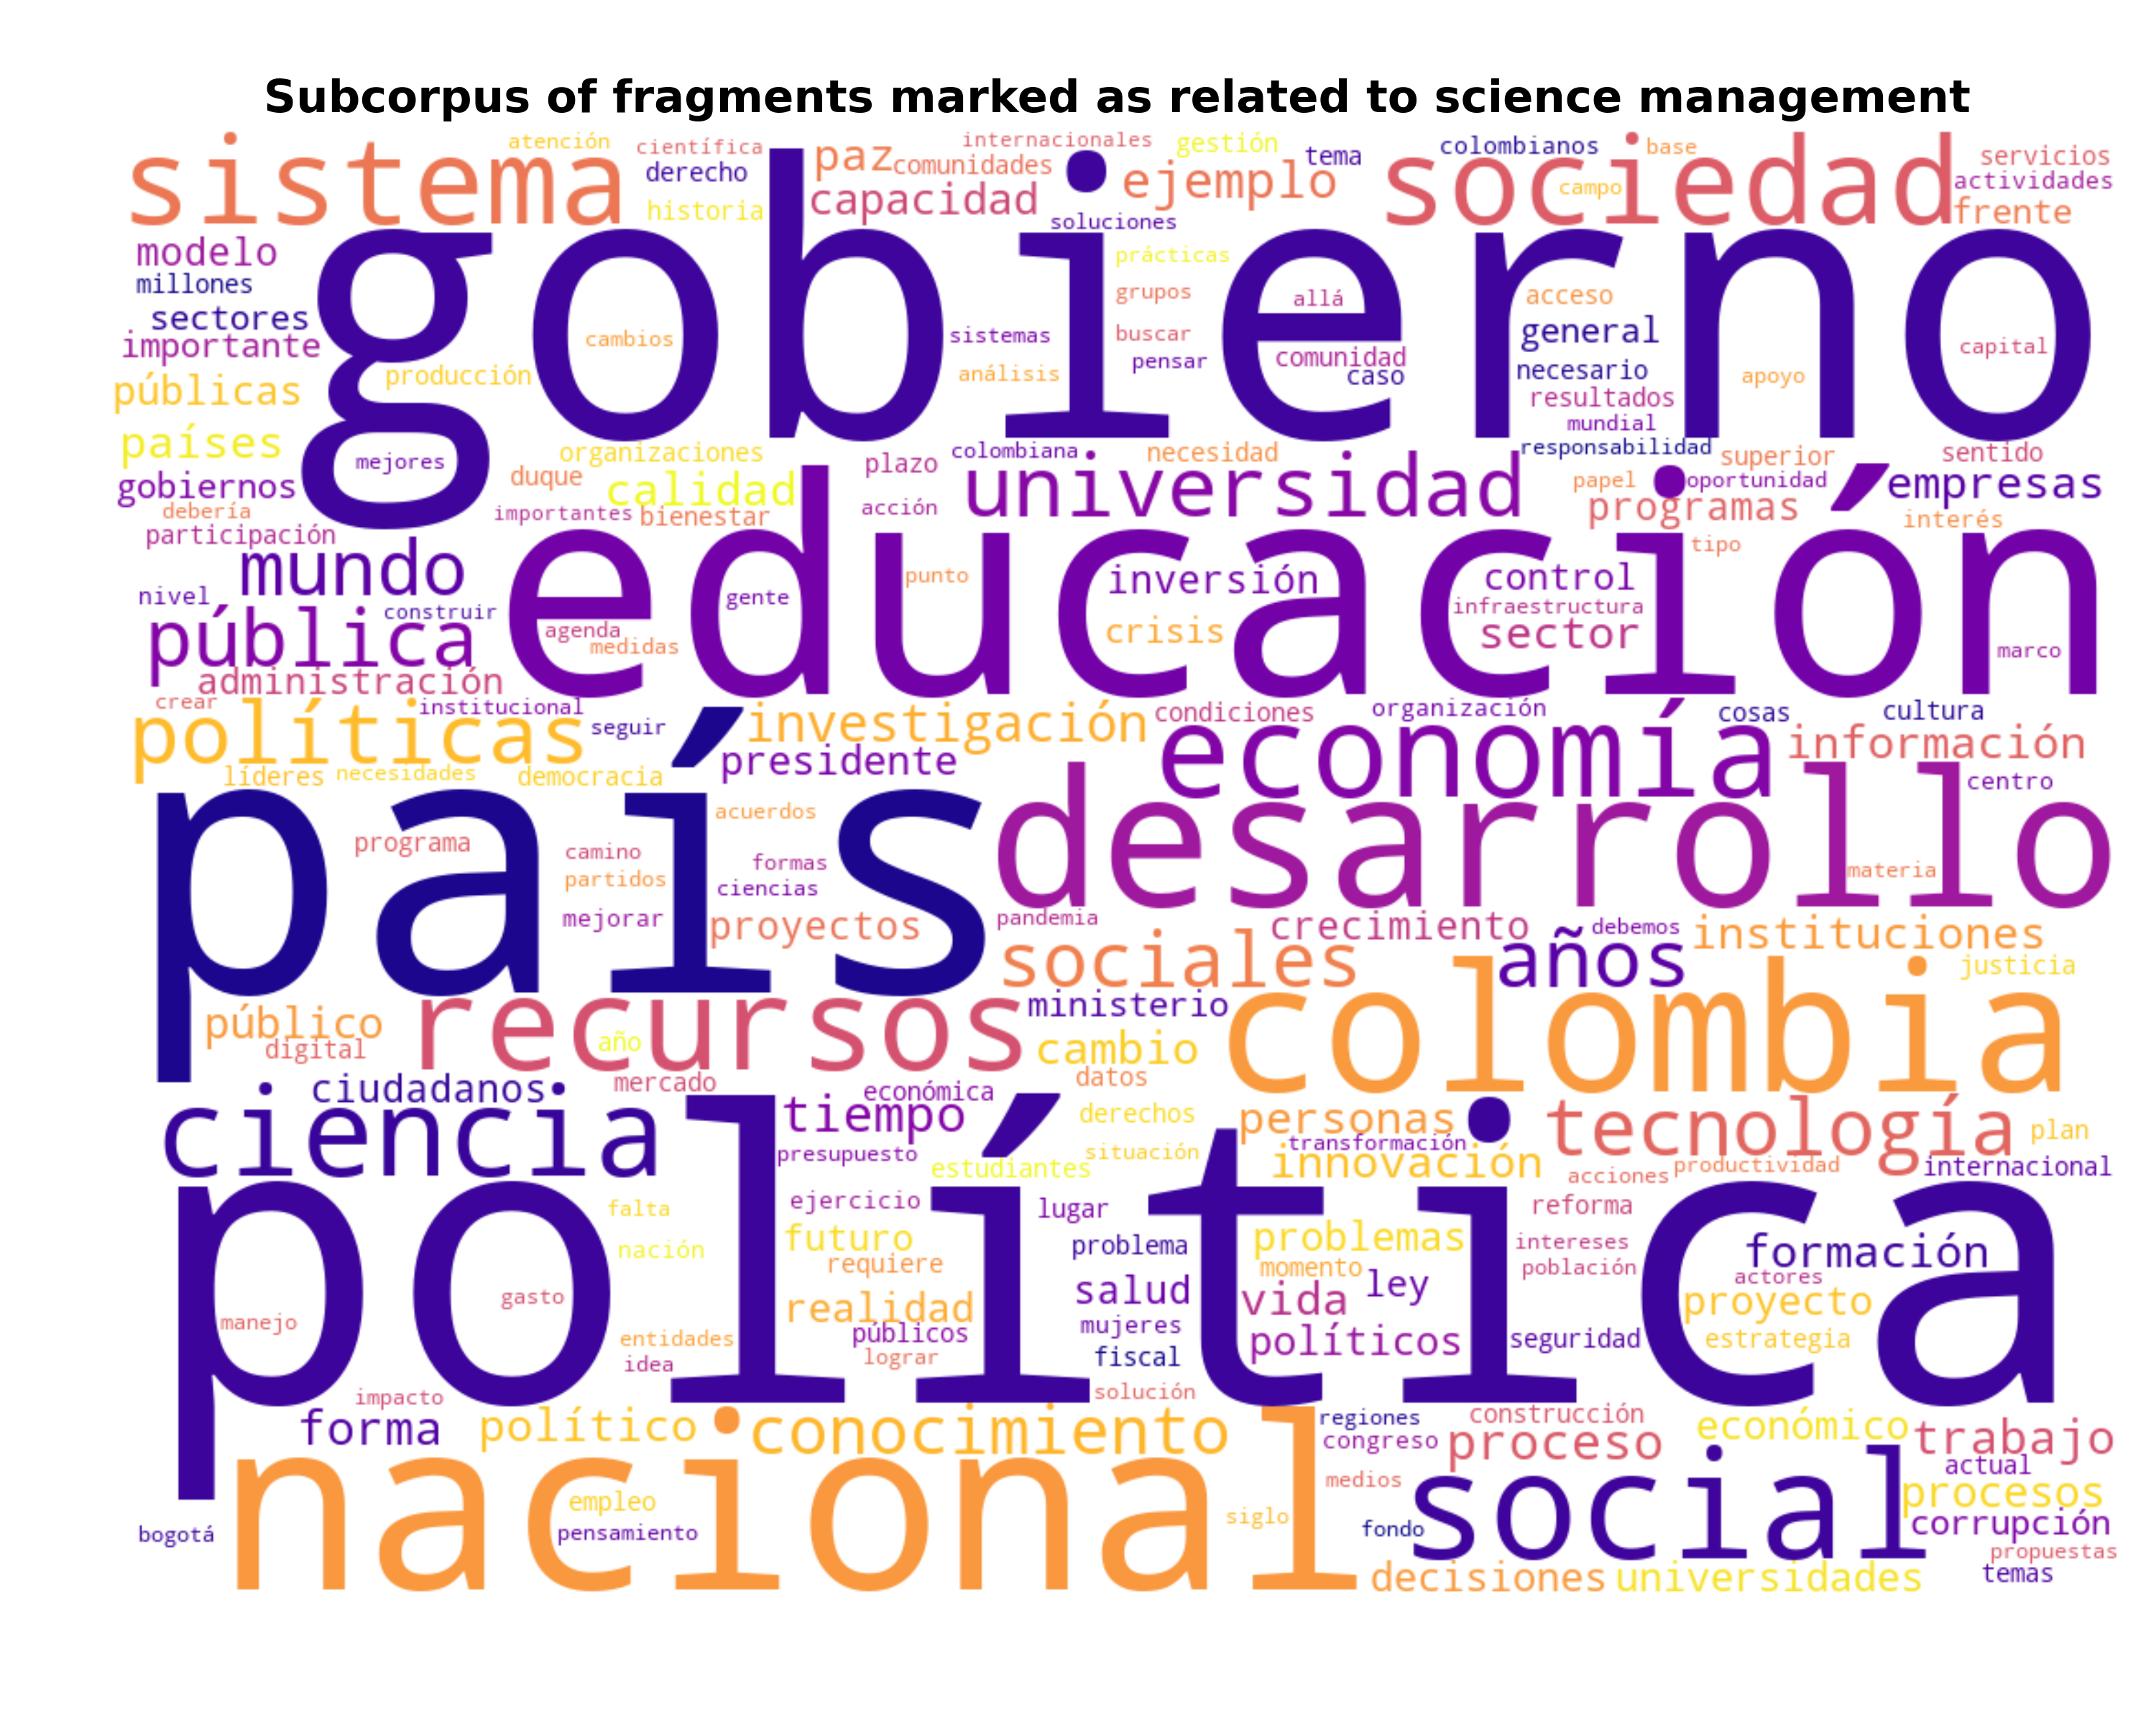
\includegraphics[width=1\textwidth]{nube_ciencia_admin.png}
	\caption{Descripción de la imagen}
	\label{fig:word_cloud_admin}
\end{figure}

\subsection{NER}

\begin{table}[H]
	\centering
	\caption{People Identified with NER}
	\label{tab:ner_people}
	\begin{tabular}{lcccccc}
		\hline
		\textbf{Entity} & \textbf{Total} & \textbf{Non-Science} & \textbf{Science} & \textbf{Science Ratio} & \textbf{Admin} & \textbf{Admin Ratio} \\
		\hline
		Mabel Torres      & 13 & 6 & 7 & 0.5385 & 7 & 0.5385 \\
		Dolly Montoya     & 12 & 8 & 4 & 0.3333 & 4 & 0.3333 \\
		Mann              & 8  & 4 & 4 & 0.5    & 3 & 0.375  \\
		Brigitte Baptiste & 8  & 3 & 5 & 0.625  & 4 & 0.5    \\
		Romer             & 8  & 2 & 6 & 0.75   & 6 & 0.75   \\
		Tharp             & 8  & 0 & 8 & 1      & 5 & 0.625  \\
		Mario Bunge       & 7  & 3 & 4 & 0.5714 & 3 & 0.4286 \\
		Alston            & 7  & 3 & 4 & 0.5714 & 4 & 0.5714 \\
		Wendy             & 6  & 3 & 3 & 0.5    & 2 & 0.3333 \\
		Echeverry         & 6  & 4 & 2 & 0.3333 & 2 & 0.3333 \\
		\hline
	\end{tabular}
\end{table}



\begin{table}[H]
	\centering
	\caption{Organizations Identified with NER}
	\label{tab:ner_organizations}
	\begin{tabular}{lcccccc}
		\hline
		\textbf{Entity} & \textbf{Total} & \textbf{Non-Science} & \textbf{Science} & \textbf{Science Ratio} & \textbf{Admin} & \textbf{Admin Ratio} \\
		\hline
		Universidad                                   & 234 & 148 & 86 & 0.3675 & 74 & 0.3162 \\
		Universidad Pedagógica Nacional              & 109 & 58  & 51 & 0.4679 & 47 & 0.4312 \\
		Colciencias                                   & 70  & 26  & 44 & 0.6286 & 42 & 0.6    \\
		Pontificia Universidad Javeriana             & 103 & 70  & 33 & 0.3204 & 31 & 0.301  \\
		Organizaciones                                & 25  & 4   & 21 & 0.84   & 21 & 0.84   \\
		University of Massachusetts Amherst           & 47  & 27  & 20 & 0.4255 & 19 & 0.4043 \\
		Ministerio de Ciencia, Tecnología e Innovación & 14  & 0   & 14 & 1      & 13 & 0.9286 \\
		ICA                                           & 33  & 19  & 14 & 0.4242 & 12 & 0.3636 \\
		Misión de Sabios                              & 25  & 10  & 15 & 0.6    & 10 & 0.4    \\
		Sistema Nacional de Innovación                & 10  & 0   & 10 & 1      & 10 & 1      \\
		Ministerio de Educación Nacional              & 28  & 18  & 10 & 0.3571 & 9  & 0.3214 \\
		Ministerio TIC                                & 28  & 18  & 10 & 0.3571 & 9  & 0.3214 \\
		DNP                                           & 24  & 15  & 9  & 0.375  & 9  & 0.375  \\
		Agencia de Desarrollo Rural                   & 20  & 11  & 9  & 0.45   & 9  & 0.45   \\
		CNA                                           & 11  & 2   & 9  & 0.8182 & 9  & 0.8182 \\
		SENA                                          & 20  & 10  & 10 & 0.5    & 8  & 0.4    \\
		UPN                                           & 15  & 6   & 9  & 0.6    & 8  & 0.5333 \\
		\hline
	\end{tabular}
\end{table}

\begin{table}[H]
	\centering
	\caption{Places Identified with NER}
	\label{tab:ner_places_institutions}
	\begin{tabular}{lcccccc}
		\hline
		\textbf{Entity} & \textbf{Total} & \textbf{Non-Science} & \textbf{Science} & \textbf{Science Ratio} & \textbf{Admin} & \textbf{Admin Ratio} \\
		\hline
		Centro                             & 17 & 8 & 9 & 0.5294 & 7 & 0.4118 \\
		Javeriana                          & 13 & 9 & 4 & 0.3077 & 4 & 0.3077 \\
		departamento de Sucre              & 11 & 7 & 4 & 0.3636 & 4 & 0.3636 \\
		Museo de Historia Natural          & 5  & 1 & 4 & 0.8    & 4 & 0.8    \\
		Océano                             & 4  & 1 & 3 & 0.75   & 3 & 0.75   \\
		Casa de la Vida                    & 3  & 0 & 3 & 1      & 3 & 1      \\
		Sede de La Paz                     & 6  & 4 & 2 & 0.3333 & 2 & 0.3333 \\
		Archivo General de la Nación       & 5  & 3 & 2 & 0.4    & 2 & 0.4    \\
		Zonas de Reserva Campesina         & 5  & 2 & 3 & 0.6    & 2 & 0.4    \\
		Columbia                           & 5  & 3 & 2 & 0.4    & 2 & 0.4    \\
		vereda la Colorada                 & 4  & 2 & 2 & 0.5    & 2 & 0.5    \\
		Pisa                               & 4  & 1 & 3 & 0.75   & 2 & 0.5    \\
		Observatorio Astronómico Nacional  & 4  & 0 & 4 & 1      & 2 & 0.5    \\
		\hline
	\end{tabular}
\end{table}

\subsection{Topic Modeling}

\begin{table}[H]
	\centering
	\caption{Topic Modeling Results}
	\label{tab:topic_modeling_results}
	\begin{tabular}{ccccp{9cm}}
		\hline
		\textbf{Topic} & \textbf{Coherence ($c_v$)} & \textbf{Percentage} & \textbf{ID} & \textbf{Keywords} \\
		\hline
		1  & 0.5668 & 16.31 & 1  & político, democracia, presidente, duque, sociedad, gobernabilidad, partidos \\
		0  & 0.6755 & 16.12 & 0  & economía, crecimiento, productividad, fiscal, empleo, inversión, rural \\
		2  & 0.6901 & 5.98  & 2  & datos, información, digital, tecnología, internet, vigilancia, seguridad \\
		4  & 0.7625 & 5.76  & 4  & universidad, formación, investigación, educación, comunidades, calidad \\
		3  & 0.5509 & 5.41  & 3  & pandemia, salud, crisis, virus, economía, cuarentena, medidas \\
		8  & 0.7162 & 4.69  & 8  & universidades, educación superior, estudiantes, públicas, sistema \\
		12 & 0.6146 & 4.13  & 12 & paz, policía, violencia, territorios, acuerdos, farc \\
		6  & 0.5937 & 4.07  & 6  & corrupción, control, funcionarios, congreso, presupuesto \\
		7  & 0.5100 & 3.82  & 7  & justicia, electoral, judicial, reforma, voto, proceso \\
		11 & 0.6974 & 3.54  & 11 & ciencia, innovación, ministerio, tecnología, colciencias, ley \\
		10 & 0.4773 & 3.41  & 10 & ciencia, pensamiento, literatura, ensayo, problemas \\
		5  & 0.7860 & 3.38  & 5  & organizaciones, estrategia, negocio, compañías, clientes \\
		9  & 0.5513 & 3.35  & 9  & ambiental, climático, biodiversidad, agua, amazonia \\
		14 & 0.5198 & 2.54  & 14 & educación superior, sena, reforma, docentes, sociedad \\
		15 & 0.5095 & 2.47  & 15 & bogotá, ciudad, alcaldía, movilidad, ciudadanos \\
		13 & 0.6523 & 2.35  & 13 & mujeres, género, equidad, violencia, sociedad \\
		16 & 0.7193 & 1.88  & 16 & estudiantes, aprendizaje, profesores, escuela, docentes \\
		17 & 0.7189 & 1.60  & 17 & trabajo, inteligencia artificial, empleo, competencias \\
		19 & 0.5968 & 1.41  & 19 & mercado, capitalismo, desigualdad, modelo económico \\
		20 & 0.4836 & 0.97  & 20 & trump, biden, diplomacia, estrategia, maduro \\
		\hline
	\end{tabular}
\end{table}

\subsection{POS-tagging}

\begin{table}[H]
	\centering
	\begin{tabular}{lrrrrr}
		\hline
		Verbos & frecuencia\_total & frecuencia\_ciencia & proporcion\_ciencia & frecuencia\_ciencia\_admin & proporcion\_ciencia\_admin \\
		\hline
		orientar     & 293 & 87 & 0,30 & 64 & 0,22 \\
		articular    & 175 & 79 & 0,45 & 62 & 0,35 \\
		coordinar    & 140 & 42 & 0,30 & 30 & 0,21 \\
		actualizar   & 122 & 37 & 0,30 & 27 & 0,22 \\
		innovar      & 83  & 23 & 0,28 & 18 & 0,22 \\
		posibilitar  & 77  & 24 & 0,31 & 21 & 0,27 \\
		maximizar    & 62  & 19 & 0,31 & 16 & 0,26 \\
		dinamizar    & 62  & 20 & 0,32 & 16 & 0,26 \\
		apalancar    & 54  & 22 & 0,41 & 17 & 0,31 \\
		posponer     & 54  & 14 & 0,26 & 14 & 0,26 \\
		cristalizar  & 53  & 13 & 0,25 & 12 & 0,23 \\
		armonizar    & 47  & 19 & 0,40 & 13 & 0,28 \\
		capacitar    & 46  & 20 & 0,43 & 13 & 0,28 \\
		\hline
	\end{tabular}
	\caption{Frecuencias y proporciones por verbos, frecuencias admin mayores a 10 y prop mayor a 0.2}
\end{table}

\begin{table}[H]
	\centering
	\begin{tabular}{lrrrrr}
		\hline
		Adjetivos & frecuencia\_total & frecuencia\_ciencia & proporcion\_ciencia & frecuencia\_ciencia\_admin & proporcion\_ciencia\_admin \\
		\hline
		científico           & 959 & 507 & 0,53 & 305 & 0,32 \\
		tecnológico          & 682 & 290 & 0,43 & 240 & 0,35 \\
		formativo            & 103 & 49  & 0,48 & 40  & 0,39 \\
		docente              & 102 & 41  & 0,40 & 38  & 0,37 \\
		inclusivo            & 98  & 36  & 0,37 & 30  & 0,31 \\
		misional             & 65  & 34  & 0,52 & 32  & 0,49 \\
		colaborativo         & 64  & 26  & 0,41 & 23  & 0,36 \\
		cuantitativo         & 56  & 24  & 0,43 & 19  & 0,34 \\
		curricular           & 50  & 21  & 0,42 & 20  & 0,40 \\
		instrumental         & 39  & 17  & 0,44 & 14  & 0,36 \\
		interdisciplinario   & 38  & 21  & 0,55 & 17  & 0,45 \\
		organizacional       & 37  & 17  & 0,46 & 14  & 0,38 \\
		gerencial            & 36  & 12  & 0,33 & 12  & 0,33 \\
		profesoral           & 36  & 15  & 0,42 & 15  & 0,42 \\
		conducente           & 31  & 13  & 0,42 & 12  & 0,39 \\
		cualificado          & 25  & 12  & 0,48 & 11  & 0,44 \\
		fitosanitario        & 24  & 12  & 0,50 & 11  & 0,46 \\
		\hline
	\end{tabular}
	\caption{Frecuencias y proporciones de adjetivos, frec admin ciencia mayor a 10, proporción mayor 0.3}
\end{table}

\begin{table}[ht]
	\centering
	\begin{tabular}{lrrrrr}
		\hline
		Sustantivos & frecuencia\_total & frecuencia\_ciencia & proporcion\_ciencia & frecuencia\_ciencia\_admin & proporcion\_ciencia\_admin \\
		\hline
		ciencia                & 1575 & 858 & 0,54 & 589 & 0,37 \\
		tecnología             & 1547 & 622 & 0,40 & 513 & 0,33 \\
		formación              & 1124 & 412 & 0,37 & 340 & 0,30 \\
		innovación             & 604  & 333 & 0,55 & 289 & 0,48 \\
		planeación             & 205  & 85  & 0,41 & 62  & 0,30 \\
		mejoramiento           & 174  & 70  & 0,40 & 53  & 0,30 \\
		fomento                & 164  & 59  & 0,36 & 50  & 0,30 \\
		doctorado              & 138  & 54  & 0,39 & 50  & 0,36 \\
		acreditación           & 93   & 64  & 0,69 & 61  & 0,66 \\
		formalización          & 93   & 33  & 0,35 & 28  & 0,30 \\
		instituto              & 89   & 36  & 0,40 & 30  & 0,34 \\
		articulación           & 88   & 41  & 0,47 & 34  & 0,39 \\
		docencia               & 59   & 22  & 0,37 & 21  & 0,36 \\
		tecnocracia            & 55   & 17  & 0,31 & 17  & 0,31 \\
		biotecnología          & 40   & 23  & 0,58 & 17  & 0,43 \\
		autoevaluación         & 39   & 25  & 0,64 & 24  & 0,62 \\
		encadenamiento         & 35   & 16  & 0,46 & 13  & 0,37 \\
		estructuración         & 35   & 13  & 0,37 & 11  & 0,31 \\
		aptitud                & 33   & 10  & 0,30 & 10  & 0,30 \\
		subsector              & 33   & 11  & 0,33 & 11  & 0,33 \\
		internacionalización   & 28   & 15  & 0,54 & 15  & 0,54 \\
		perdurabilidad         & 26   & 18  & 0,69 & 14  & 0,54 \\
		conceptualización      & 18   & 14  & 0,78 & 14  & 0,78 \\
		subsistema             & 16   & 12  & 0,75 & 11  & 0,69 \\
		\hline
	\end{tabular}
	\caption{Frecuencias y proporciones de sustantivos, frecuencias mayor a 10 para admin, proporción mayor a 0,3}
\end{table}


\clearpage






\section{CONCLUSIONES}

\bibliographystyle{apsrev4-2}
\bibliography{bibliografia} % Incluya la bibliografía en el archivo: bibliografia.bib

\end{document}
